\section{Experiments}
\subsection{Setup}
\label{sec:experimental-setup}

\begin{table*}[t]
\centering
\caption{Development prediction. Neural results average three seeds; CIs use 2,000 participant resamples. Within: mean within-participant AUROC. Bold/underlined: best/second distinct displayed score; gray: HNE.}
\label{tab:main}
\hnetable{tables/main}
\end{table*}

\paragraph{Cohorts and splits.}
RESILIENT and BrisT1D-Open provide participant-disjoint development evaluations \citep{hneD02,hneD03,hneD04}. Both yield ten daily state coordinates from physiological and behavioral measurements and one context coordinate: steps for RESILIENT, carbohydrate intake for BrisT1D. Each state contributes a daily mean and standard deviation when four hourly observations are available. Five fixed participant folds rotate through evaluation, with the next fold for validation and the other three for training.

Human Rhythms \citep{hneD07} and College Experience \citep{hneD08} provide separately held-out participant tests. Identifier hashes fix training/validation/test splits before outcome construction; models are frozen before generating test endpoints. Human Rhythms supplies ten state and five site-weather coordinates; College supplies nine state and four context coordinates. Eligible training/validation/test counts are 85/28/28 and 126/44/41 people, respectively. Their test sets contain 2,980 and 15,137 origins. Appendix~\ref{app:reproducibility} specifies fields, available versus eligible people, and recording durations.

The development cohorts yield 1,990/1,238 origins from 56/19 participants, with 317/152 positives.

\paragraph{Comparators.}
We rerun dynamical network biomarker (DNB), the released FCM and CATCH cores \citep{hneH01,hneC01}, history logistic regression and histogram gradient boosting (HGB), and alternative HNE heads. FCM and CATCH retain their predictive/reconstruction objectives and run all 20 epochs for each of three fixed seeds. Ensembles average validation-negative percentile-transformed scores. JAPE retains its forecasting backbone and dual-view alerting head \citep{hneP02}, adapted to the same future interval; we report both native validation-F1 and validation-AUROC checkpoint selection. Every method uses historical inputs at inference and the same future labels for evaluation. Architecture, optimization, and score adapters appear in Appendix~\ref{app:reproducibility}.

\paragraph{Metrics and transfer.}
Primary comparisons use common scoreable origins: 1,964/1,230 for development and 2,948/14,963 for the held-out cohorts. Development AUROC averages fold-specific AUROCs weighted by positive--negative pair counts; held-out tests use global AUROC. We report 2,000 participant-bootstrap percentile intervals, paired differences, within-person AUROC, average precision, and validation-selected operating points. Strongest-control intervals reselect the best comparator within each resample. Transfer freezes the feature definitions and distinguishes source-only scoring, target-only fitting, transfer of the source basis, and a source-coefficient prior. CARE and ESA use their native fault and expert-event endpoints; all endpoint and split definitions are specified before their evaluations.

Three research questions organize the evaluation:
\begin{description}
\item[RQ1] Which changes in multivariate rhythms precede sustained disturbances relative to an individual's usual fluctuations?
\item[RQ2] Can jointly learning personal history, indicator relationships, and observed context improve advance disturbance warning?
\item[RQ3] Can a shared warning rule transfer across domains with different variables and disturbance endpoints?
\end{description}

\begin{figure*}[t]
\centering
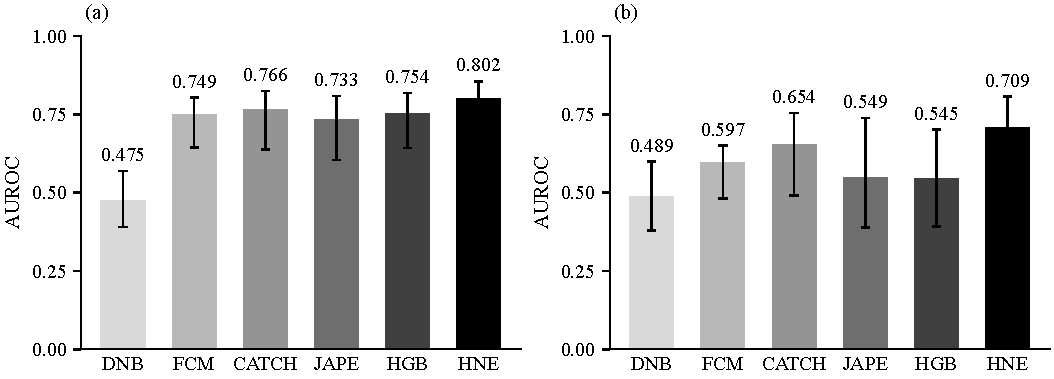
\includegraphics[width=\textwidth]{figures/main_auroc.pdf}
\caption{Development AUROC: (a) RESILIENT; (b) BrisT1D-Open. Error bars are participant-bootstrap 95\% intervals. JAPE uses validation-AUROC selection.}
\label{fig:main}
\end{figure*}
